\documentclass{article}
\usepackage[utf8]{inputenc}
\usepackage{graphicx}
\begin{titlepage}
\begin{center}

\large{\textbf{North South University}}

\large{Department of Electrical \& Computer Engineering} 

\vspace{1cm}


\LARGE{{CSE311-Database Project}} 

\large{Title of the Project: House Rental Management System}

\paragraph{}
Course: CSE311
 
Faculty: Intisar Tahmid Naheen (ITN)
 
Lab-instructor: Nazmul Alam Dipto
 
Semester: Summer-2021


\vspace{1cm}

\end{center}




\normalsize{\textbf{Submitted by:}} 

\vspace{0.5cm}

Name: Samil Abdullah

ID: 1611408642
\vspace{0.5cm}

Name: Sazzad Alam 

ID: 1611200642


\vspace{0.5cm}
\normalsize{Submission date:09.07.21} 






\end{titlepage}



\begin{document}

\section{Introduction}

House Rental Management System is a platform where a person can easily find a suitable house within his requirements (Price, Number of bedrooms, Number of Toilets, Common Space etc.). When a tenant fills up his requirements through website, the website will show some suggest house which can be suitable for him. He can also message the owner for confirmation. After that the tenant can pay all the bills including house rent from this platform including Bkash / Rocket. The tenant can also complain about anything about his apartment through this website. The tenant has to upload all his information and document through this website before 1 month of rent a house. An owner of a house can upload his requirements to rent his house. He can upload his appointment picture and upload it through website. He can show all the information of the tenant and he can show all the transaction history of payment.

\vspace{3cm}


\section{Software Use}

We will use: 

1.	VS Code

2.	Adobe Photoshop

3.	Flask Framework for backend 

4.	SQLite for database 

VS Code is for writing the code of HTML, CSS, FLASK and all. We are used Photoshop for some background image. SQLite is used for local hosting server. 
\vspace{5cm}
\section{Use Case Diagram:}

Our project use case diagram looks like this.
\begin{center}
    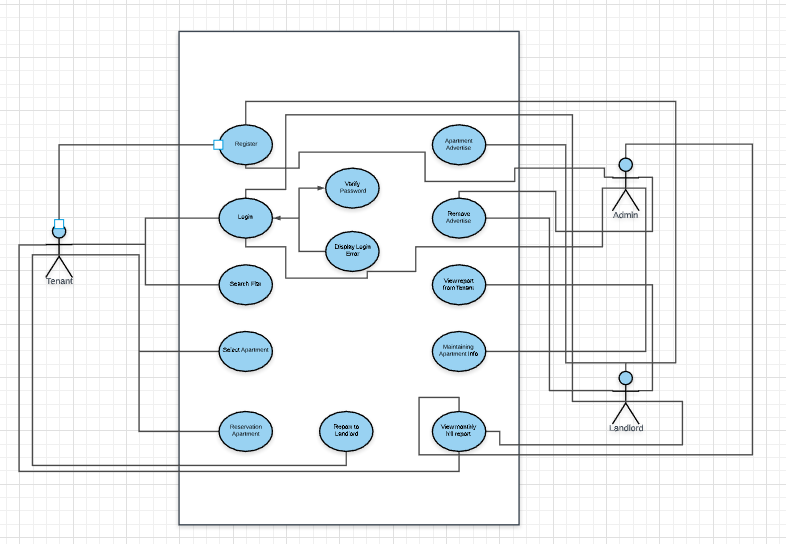
\includegraphics[width=\linewidth]{flow_chart.png}
\end{center}

\vspace{5cm}

\section{Expected Outcomes:}
We expect to endure better House Rental site for the Bangladeshi peoples. In future people can study about our project and they can add more plans to our project so that we can update more.

\end{document}
